\section{Forma normalna rekursji}
\begin{theorem}[O formie normalnej rekursji]
    Istnieje funkcja \( U: \natural \to \natural \), \( U \in PRec \) oraz predykaty \( \tau^n \in \natural^{n+2} \) z \( PRec \), takie że dla każdej funkcji \( f: \natural^n \to \natural \in Rec \)
    \begin{itemize}
        \item \( \forall_{x_1, \dots, x_n} \exists_y \ \tau^n(e_f,x_1,\dots,x_n,y) \)
        \item \( f(x_1, \dots, x_n) = U\big(\mu y [\tau^n(e_f,x_1,\dots,x_n,y)]\big) \)
    \end{itemize}
    Liczba \(y\) to numer obliczenia funkcji o numerze \(e_f\) na wejściu \(\vec{x}\). Wtedy \( \mu y [\tau^n(e_f,\vec{x},y)] \) znajduje numer tej historii obliczeń, a \(U\) odzyskuje z niej wynik.
\end{theorem}
\begin{proof}
    Definiujemy drzewa obliczeń funkcji \( f \):
    \begin{itemize}
    \singlespacing
        \item Liście: \( \ f(x) = 0, \  f(x) = x+1, \ f(\vec{x}) = x_k \ \) dla funkcji inicjujących
        \item Drzewo dla złożenia \( f(\vec{x}) = g(h_1(\vec{x}),\dots h_k(\vec{x})) \):
        \begin{figure}[H]
          \centering
          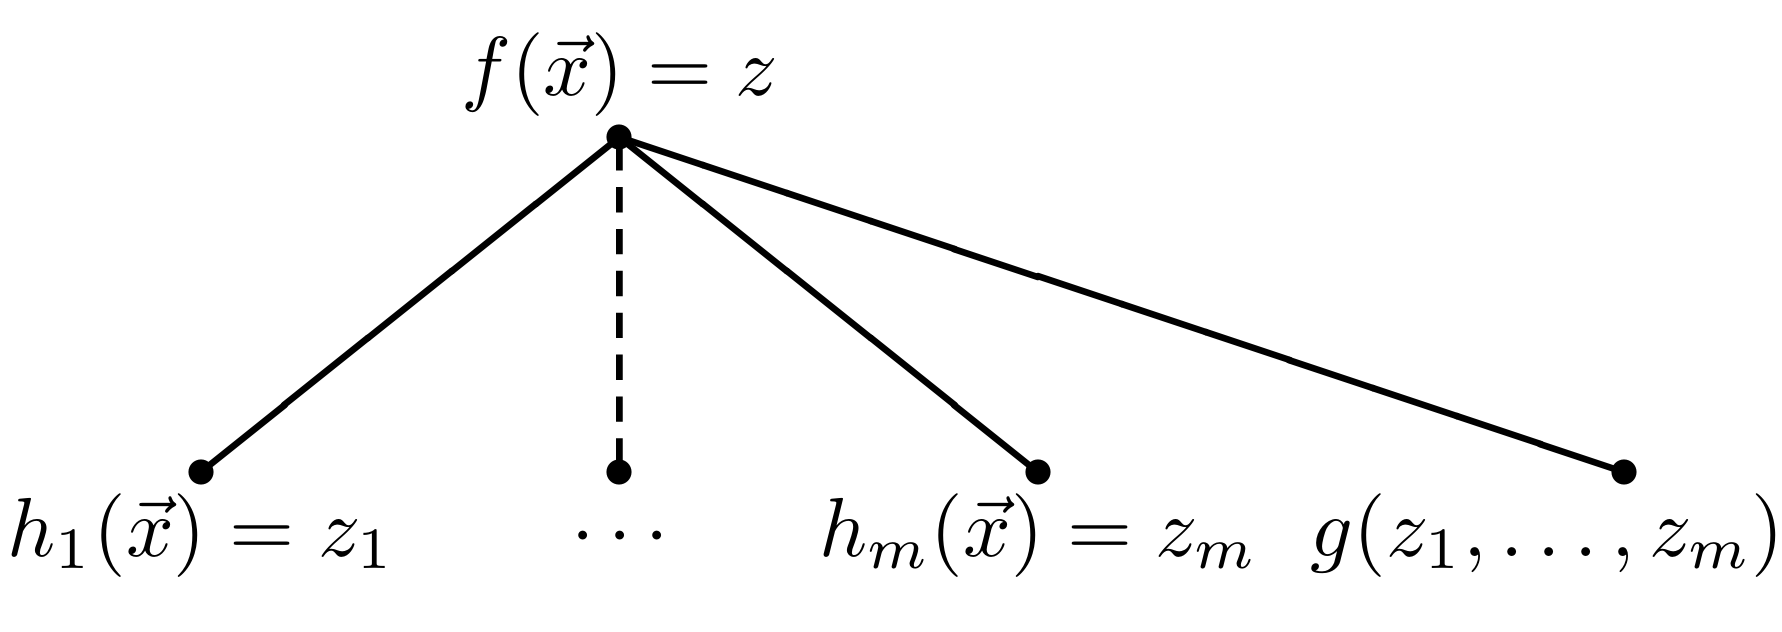
\includegraphics[width=0.55\textwidth]{img/tree_composition}
        \end{figure}
        \newpage
        \item Drzewo obliczeń dla rekursji prostej
        \begin{figure}[H]
          \centering
          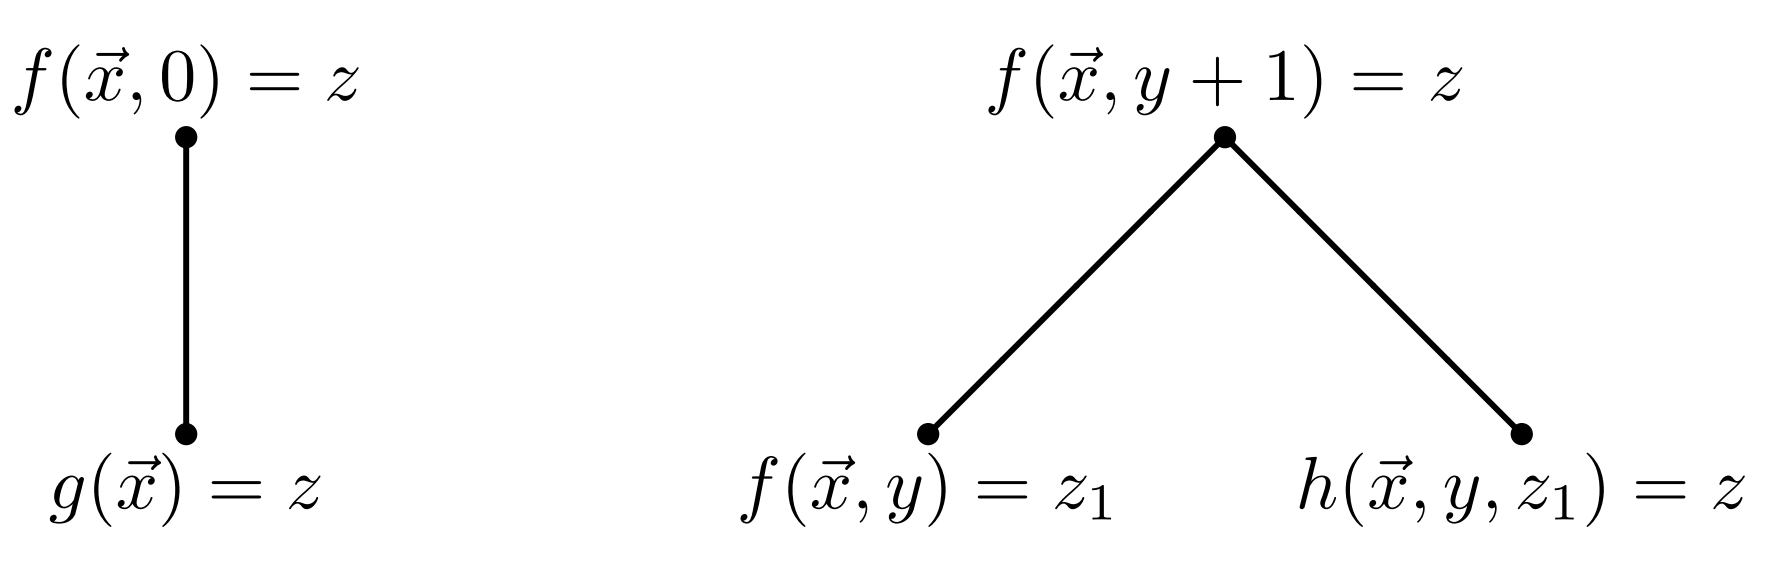
\includegraphics[width=0.55\textwidth]{img/tree_recursion}
        \end{figure}
        \item Drzewo dla \(\mu\)-rekursji
        \begin{figure}[H]
          \centering
          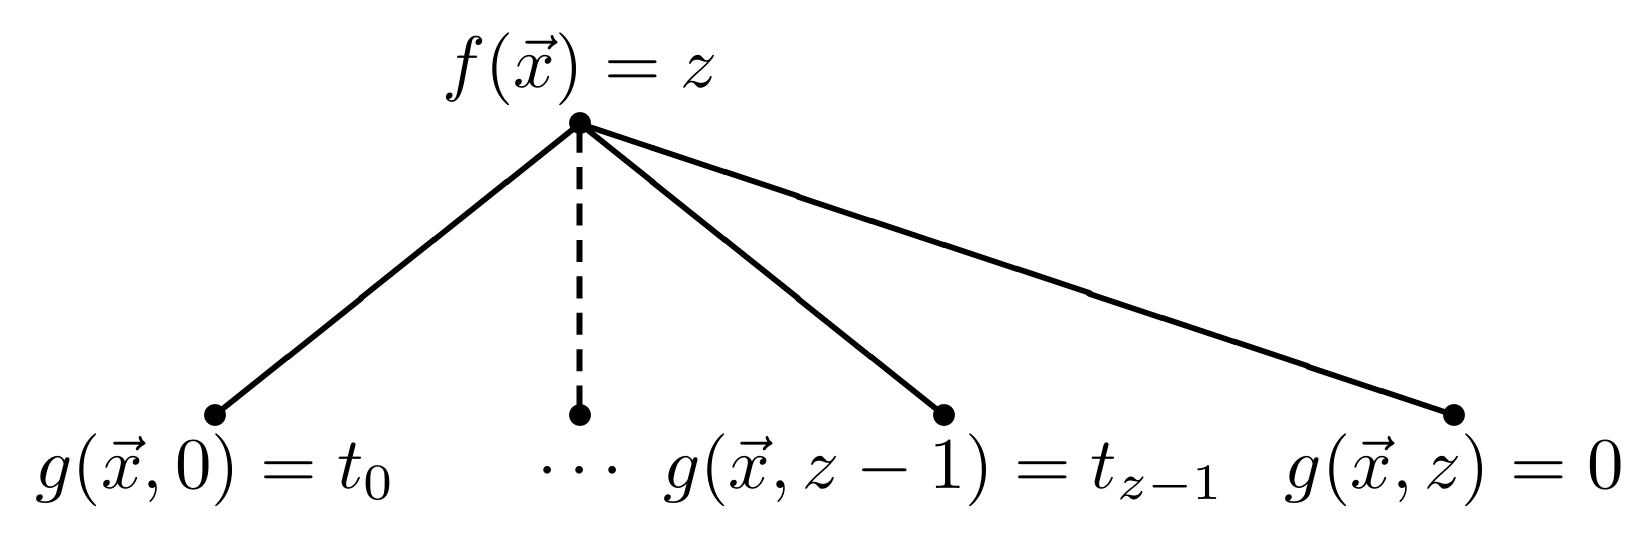
\includegraphics[width=0.55\textwidth]{img/tree_mu_operator}
        \end{figure}
    \end{itemize}
    Pozostało tylko ponumerować drzewa.
    Wierzchołek \(v\):
    \[ v=[f(x_1,\dots,x_n)=z] \]
    numerujemy jako:
    \[ \hat{v}=\langle e_f,\langle x_1,\dots,x_n \rangle,z \rangle \]
    \begin{figure}[H]
        \centering
        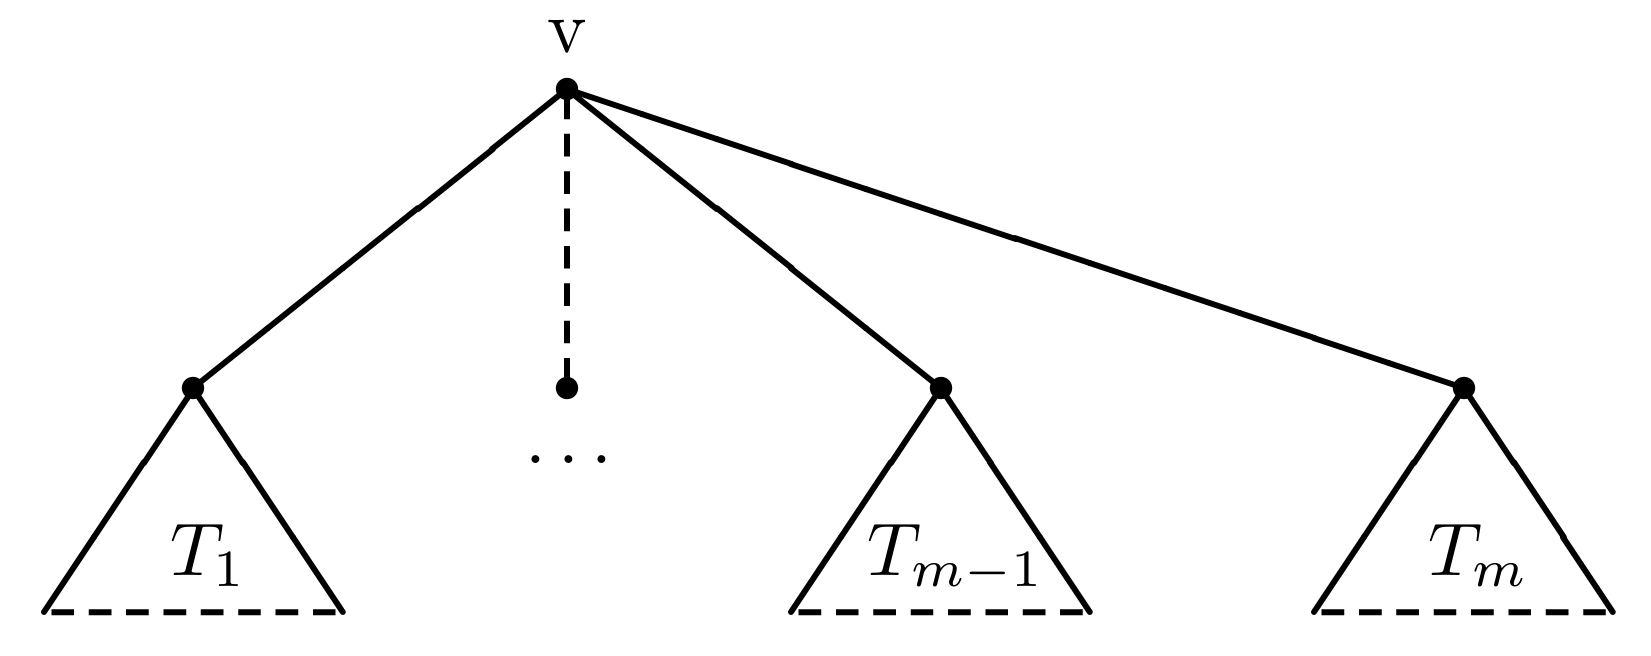
\includegraphics[width=0.5\textwidth]{img/tree}
    \end{figure}
    Drzewa kodujemy jako \( \hat{T}=\langle \hat{v},\hat{T}_1,\dots, \hat{T}_k \rangle) \)

    Konstruujemy predykat \( \mathcal{T}(y) \in Prec \) rozumiany jako \textit{\( y \) jest kodem drzewa obliczeń}.

    \( A(y) \) -- wstępne warunki
    
    \[ A(y) = \underbrace{\seq(y)}_{\text{kod drzewa}} \land \underbrace{\seq((y)_1) \land \big(\length((y)_1) = 3\big)}_{\text{kod } v} \land \underbrace{\seq((y)_{1,1})}_{\text{kod } f} \land \underbrace{\seq((y)_{1,2})}_{\text{argumenty}} \]
    \( B(y) \) -- warunki poprawnego kodowania funkcji inicjujących \\
    \( C(y) \) -- warunki poprawnego kodowania złożenia \\
    \( D(y) \) -- warunki poprawnego kodowania rekursji prostej \\
    \( E(y) \) -- warunki poprawnego kodowania \( \mu \)-operatora

    Korzystając z powyższych definiujemy predykat \( \mathcal{T} \) jako:
    \begin{align*}
        & \mathcal{T}(y) \iff \\
        & A(y) \ \land & \text{(poprawność kodu)} \\
        & \big[ B(y) \lor C(y) \lor D(y) \lor E(y) \big] \ \land & \text{(dopasowanie którejś z dopuszczalnych funkcji)} \\
        & \big[ \length(y) > 1 \rightarrow \forall_{2 \leq i \leq \length(y)} \ T(y(i)) \big] & \text{(poprawność poddrzew)} \\
    \end{align*}
    Odwołanie do \( \mathcal{T}(y(i)) \) nie jest problemem, bo możemy korzystać z rekursji z historią, a~\( y(i) <  y \).

    W ten sposób otrzymujemy \(\tau^n, U \in \prec\):
    \begin{align*}
        & \tau^n(e_f, \vec{x}, y) = \\
        & \mathcal{T}(y) \ \land \\
        & \big[ (y)_{1,1} = e_f \big] \ \land & \text{(poprawny numer funkcji)} \\
        & \big[ (y)_{1,2} = \langle \vec{x} \rangle \big] & \text{(zgodność argumentów)} \\ \\
        & U(y) = (y)_{1,3}
    \end{align*}
\end{proof}